\usetikzlibrary{arrows.meta}
% id: 2002_shanghai_liberal_q13_fig1; family: basic_conic
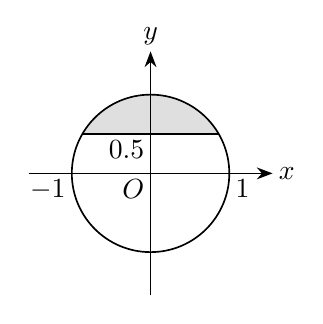
\begin{tikzpicture}[x=1cm,y=1cm,line width=.6pt,font=\normalsize,every node/.style={inner sep=0pt},>=Stealth]
\fill[gray!25] (-0.8660254037844386,0.5)--(0.8660254037844386,0.5) arc[start angle=30,end angle=150,radius=1cm]--cycle;
\draw[->] (-1.55,0)--(1.55,0) node[right,inner sep=0pt,xshift=2pt] {$x$};
\draw[->] (0,-1.55)--(0,1.55) node[above,inner sep=0pt,yshift=2pt] {$y$};
\draw (0,0) circle[radius=1cm];
\draw (-0.8660254037844386,0.5)--(0.8660254037844386,0.5);
\node[anchor=north east,inner sep=0pt,xshift=-2pt,yshift=-2pt] at (0,0) {$O$};
\node[anchor=north east,inner sep=0pt,xshift=-2pt,yshift=-2pt] at (-1,0) {$-1$};
\node[anchor=north west,inner sep=0pt,xshift=2pt,yshift=-2pt] at (1,0) {$1$};
\node[anchor=north east,inner sep=0pt,xshift=-2pt,yshift=-2pt] at (0,0.5) {$0.5$};
\end{tikzpicture}
